\chapter{\label{ch7-performance}Camera Performance} 

\minitoc

\section{Introduction}

As discussed in Chapter~\ref{ch3-architecture}, it is important that the \gls{chec} camera meets certain criteria in order for it to be accepted as an in-kind contribution to \gls{cta}. One important subset of the criteria is the camera's performance. The requirements that must be fulfilled are driven by the science goal of \gls{cta}. If a camera does not meet the requirements laid out by the \gls{cta} observatory, then it will be refused as a contribution in its current state, lest the science goals of \gls{cta} are not achieved.

This chapter will cover many of the primary standards used to assess a \gls{cta} camera's performance. The results shown in this chapter are all my own, and are obtained using the procedures defined in the preceding chapters. Two important aspects of the camera's performance which are not included in this chapter are the trigger efficiency and absolute photon detection efficiency. The investigations into these parameters are ongoing, of which I have not had direct involvement with as part of my DPhil.

\section{CHEC-S Monte Carlo Model}

An important preface to reporting on the performance of \gls{chec} is the description of the efforts in generating an accurate model of the camera for use inside the Monte Carlo simulations performed by \pkg{sim\_telarray} (Chapter~\ref{ch4-software}). These simulations allow us to more widely explore the parameter space related to our camera performance, and identify potential issues that cause the real camera to drift away from ideal operation. It is also a necessary step in investigating the on-sky performance of the telescope, as:

\begin{itemize}
\item One does not have prior knowledge of the properties of the light incident on the pixels in the real world.
\item The camera is still being tested in the lab. An on-sky campaign for \gls{chec-s} on the \gls{astri} telescope structure is planned for later this year.
\end{itemize}

Contained within the lab data are the parameters required for the Monte Carlo validation process. Important parameters include:

\begin{itemize}
\item Pixel position on the focal surface,
\item Pulse shape for a single photoelectron,
\item Trigger discrimination behaviour,
\item Quantum efficiency (or \gls{pde}),
\item Variation of quantum efficiency between pixels
\item Electronic baseline variation,
\item Photosensor gain,
\item Variation of gain between pixels,
\item \gls{spe} spectrum shape.
\end{itemize}

\begin{figure}
	\centering
%     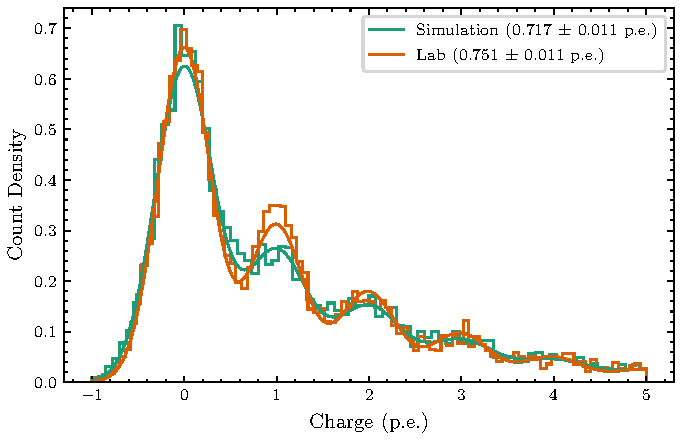
\includegraphics[width=\textwidth]{spe_sim_lab} 
	\caption[Comparison of the SPE spectra between lab measurements and simulations.]{Comparison of the SPE spectra for a single pixel between lab measurements and simulations after an initial attempt towards a more accurate Monte Carlo model. The SPE spectra are identically extracted in both cases, using the \textit{Cross Correlation} charge extraction method. Both spectra are normalised in the x direction by their respective single-photoelectron value, and in the y direction such that their integral is 1.}
	\label{fig:spe_sim_lab}
\end{figure}

\begin{table}[h!]
\centering
\begin{tabular}{ll|ll} \toprule
    Fit Parameter        &            & Simulation & Lab    \\ \midrule
    Average Illumination & [\si{\pe}] & 0.717      & 0.751  \\
    Pedestal Deviation   & [\si{\pe}] & 0.314      & 0.286  \\
    Gain Deviation       & [\si{\pe}] & 0.109      & 0.0783 \\
    Optical Crosstalk    &            & 0.387      & 0.350  \\ \bottomrule
\end{tabular}
\caption{Parameter values resulting from the fit to the spectra in Figure~\ref{fig:spe_sim_lab}}
\label{table:spe_sim_lab}
\end{table}

For the simulation results presented in this thesis, an updated value was obtained for as many of the relevant \pkg{sim\_telarray} parameters as possible. Figure~\ref{fig:spe_sim_lab} displays the resulting differences in terms of the \gls{spe} spectra between lab and simulation. The discrepancies in parameters resulting from the fits to the \gls{spe} spectra are shown in Table~\ref{table:spe_sim_lab}, and are deemed to be close enough for the investigations in this thesis. Further details about the fit procedure for \gls{spe} spectra can be found in Appendix~\ref{a1-spe}. The differences between lab and simulation in other factors and at higher amplitudes are explored through \textit{Charge Resolution} comparisons, investigated later in this chapter.

\section{CHEC-S Charge Resolution}

The \textit{Charge Resolution} is the principle criterion used within \gls{cta} to express how well the camera can resolve a signal. The concept of \textit{Charge Resolution} is introduced in Section~\ref{section:cr}, alongside the \gls{cta} requirement \requirementref{B-TEL-1010 Charge Resolution}. It not only measures the quality of the camera's photosensor and electronics, but also the aptitude of the calibration and signal extraction. Consequently, obtaining a \textit{Charge Resolution} of the camera that meets this requirement has been the underlying driver behind my efforts in developing the techniques described in this thesis.

\subsection{Procedure and Datasets}

As directed in the \requirementref{B-TEL-1010 Charge Resolution} requirement, one must validate \textit{Charge Resolution} results in three ways. To achieve this, and understand the relationship between the three validation approaches, four procedures are used to obtain a \textit{Charge Resolution}. The procedures, and their associated name for the purpose of this thesis, are:

\begin{description}
\item [Lab] .
\item [MCLab] .
\item [MCLabTrue] . 
\item [MCOnsky] .
\end{description}


\begin{enumerate}
\item 
\end{enumerate}


MCLab has perfect uniform illumination

\subsection{Lab Results}

\notes[inline,caption={}]{
	\begin{itemize}
		\item Measured versus True
        \item Average versus True
        \item Charge resolution
        \item Charge resolution / Requirement
        \item Justification of the lab chargeres using equation with ENF
	\end{itemize}
}

\subsection{Lab versus Monte Carlo}

\notes[inline,caption={}]{
	\begin{itemize}
		\item Differences between Lab and MC
        \begin{itemize}
			\item Saturation
            \item TFs
            \item Timing
            \item Electrical Crosstalk
            \item OPCT
            \item Reference Pulse shape
            \begin{itemize}
            	\item Can see change in FWHM
        		\item CE investigation excludes this contribution though
			\end{itemize}
		\end{itemize}
        \item 
	\end{itemize}
}
\notes[inline]{Remember to talk about how the MC charge resolution provides us insight into performance with perfect Transfer Functions}
\notes[inline]{big diff between MC and the lab is the potential cross talk in the electronics and the effect e.g. of ground bounce - difference in full camera illumination}

\subsection{Night Sky Background}

\notes[inline,caption={}]{
	\begin{itemize}
		\item MCLab
        \item MCOnsky
	\end{itemize}
}

\subsection{Optical Crosstalk}

\notes[inline,caption={}]{
	\begin{itemize}
		\item MC
        \item Changing bias voltage - meets requirements, but at the cost of cherenkov shower resolution, reference ch3. Need to reduce opct without reducing bias voltage - better detectors
	\end{itemize}
}

\subsection{Conclusion}

\notes[inline,caption={}]{
	\begin{itemize}
		\item Can we meet requirement with lower opct? show with enf equation at 125 MHz
	\end{itemize}
}

\section{CHEC-S Pulse Shape}

\section{CHEC-S Time Resolution}

\section{CHEC-M}

\notes[inline]{Comparison in performance between CHEC-M and CHEC-S. show SPE spectrum again, huge decrease in spe\_sigma}



